%% ============================================================
%% inception-mcp — Présentation du projet
%% Compiler : pdflatex slides.tex
%% ============================================================
\documentclass[aspectratio=169, 10pt]{beamer}

\usetheme{metropolis}
\setbeamertemplate{frame numbering}[fraction]

\usepackage[utf8]{inputenc}
\usepackage[T1]{fontenc}
\usepackage[english]{babel}
\usepackage{booktabs}
\usepackage{tabularx}
\usepackage{xcolor}
\usepackage{listings}
\usepackage{fontawesome5}
\usepackage{hyperref}
\usepackage{tikz}

\definecolor{inc-blue}{HTML}{2E4057}
\definecolor{inc-teal}{HTML}{048A81}
\definecolor{inc-orange}{HTML}{E76F51}
\definecolor{inc-green}{HTML}{57A773}
\definecolor{inc-gray}{HTML}{6C757D}

\setbeamercolor{frametitle}{bg=inc-blue, fg=white}
\setbeamercolor{progress bar}{fg=inc-teal}
\setbeamercolor{alerted text}{fg=inc-orange}

\lstset{
  basicstyle=\ttfamily\footnotesize,
  backgroundcolor=\color{gray!10},
  frame=single, framerule=0pt,
  breaklines=true, columns=flexible,
  keepspaces=true,
}

\newcommand{\done}{\textcolor{inc-green}{\faCheckCircle}}

\title{inception-mcp}
\subtitle{MCP Server \& CLI for INCEpTION}
\author{Raphaël Faure}
\date{March 2026}
\institute{\url{https://github.com/RaphFaure/inception-mcp}}

\begin{document}

\maketitle

%% --------------------------------------------------------
\begin{frame}{What is inception-mcp?}

  \textbf{INCEpTION} is an open-source web platform for NLP annotation
  (text spans, relations, dependency graphs). It exposes a REST API (AERO v1).

  \bigskip
  \textbf{inception-mcp} provides two interfaces to that API:

  \begin{columns}
    \begin{column}{0.48\textwidth}
      \begin{block}{MCP server}
        Exposes INCEpTION operations as \textbf{tools for AI agents}
        (Claude Code, Claude Desktop).\\[4pt]
        \faRobot\; Ask Claude: \textit{``upload all my texts to project 1''}
      \end{block}
    \end{column}
    \begin{column}{0.48\textwidth}
      \begin{block}{CLI}
        Same operations as \textbf{shell commands},
        no AI agent required.\\[4pt]
        \faTerminal\; \texttt{inception-cli upload --project 1 --file doc.txt}
      \end{block}
    \end{column}
  \end{columns}

  \bigskip
  Both share a single \texttt{InceptionClient} layer — one codebase, two entry points.
\end{frame}

%% --------------------------------------------------------
\begin{frame}{Motivation}

  \textbf{Problem:} Uploading and managing dozens of annotation documents in INCEpTION
  manually (via the web UI) is repetitive and error-prone at corpus scale.

  \bigskip
  \textbf{Use case (DB\_narratives thesis):}
  \begin{itemize}
    \item 87,485 clauses across 18 texts to annotate for SFL process types
    \item Need to upload batches of documents, track annotation state, export results
    \item Want Claude Code to orchestrate the annotation pipeline end-to-end
  \end{itemize}

  \bigskip
  \textbf{Solution:} wrap the AERO v1 REST API as MCP tools so that both
  a human (CLI) and an AI agent (MCP) can drive INCEpTION programmatically.
\end{frame}

%% --------------------------------------------------------
\begin{frame}{Architecture}

  \begin{center}
  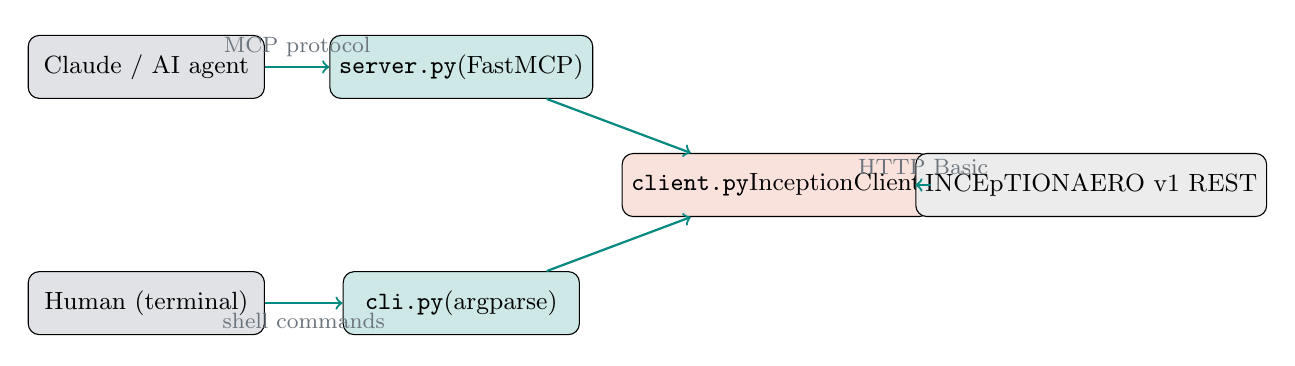
\begin{tikzpicture}[
    box/.style={draw, rounded corners, fill=white, minimum width=3cm,
                minimum height=0.8cm, font=\small},
    arr/.style={->, thick, inc-teal},
    lbl/.style={font=\footnotesize, inc-gray},
  ]
    % Clients
    \node[box, fill=inc-blue!15] (claude) at (-4, 1.5) {Claude / AI agent};
    \node[box, fill=inc-blue!15] (human)  at (-4,-1.5) {Human (terminal)};

    % Interfaces
    \node[box, fill=inc-teal!20] (server) at (0, 1.5) {\texttt{server.py}\\(FastMCP)};
    \node[box, fill=inc-teal!20] (cli)    at (0,-1.5) {\texttt{cli.py}\\(argparse)};

    % Core
    \node[box, fill=inc-orange!20, minimum width=3cm] (client) at (4, 0)
          {\texttt{client.py}\\InceptionClient};

    % INCEpTION
    \node[box, fill=gray!15, minimum width=3cm] (inception) at (8, 0)
          {INCEpTION\\AERO v1 REST};

    % Arrows
    \draw[arr] (claude)  -- node[lbl, above]{MCP protocol} (server);
    \draw[arr] (human)   -- node[lbl, below]{shell commands} (cli);
    \draw[arr] (server)  -- (client);
    \draw[arr] (cli)     -- (client);
    \draw[arr] (client)  -- node[lbl, above]{HTTP Basic} (inception);
  \end{tikzpicture}
  \end{center}
\end{frame}

%% --------------------------------------------------------
\begin{frame}[fragile]{8 MCP Tools}

  \begin{columns}
    \begin{column}{0.5\textwidth}
      \textbf{Projects}
      \begin{lstlisting}
list_projects()
create_project(name, description?)
delete_project(project_id)
      \end{lstlisting}

      \textbf{Documents}
      \begin{lstlisting}
list_documents(project_id)
upload_document(project_id,
    file_path, fmt?)
delete_document(project_id,
    document_id)
      \end{lstlisting}
    \end{column}
    \begin{column}{0.5\textwidth}
      \textbf{Annotations}
      \begin{lstlisting}
list_annotations(project_id,
    document_id)
export_annotations(project_id,
    document_id, user,
    fmt?,  output_path?)
      \end{lstlisting}

      \smallskip
      \textbf{13 export formats:}\\
      \footnotesize
      ctsv3, xmi, xmi-struct,\\
      conllu, conll2003/2006/2009/2012,\\
      text, tcf, jsoncas,\\
      jsoncas-struct, nif
    \end{column}
  \end{columns}
\end{frame}

%% --------------------------------------------------------
\begin{frame}[fragile]{CLI — Quick Reference}

\begin{lstlisting}[basicstyle=\ttfamily\scriptsize]
# List projects
inception-cli list-projects

# Upload a document
inception-cli upload --project 1 --file narrative_douglass.txt --format text

# List documents in a project
inception-cli list-documents --project 1

# Export annotations (ctsv3 to file)
inception-cli export --project 1 --doc 42 --user admin --format ctsv3 --out annot.tsv

# Export to stdout (pipe-friendly)
inception-cli export --project 1 --doc 42 --user admin --format xmi
\end{lstlisting}

  \bigskip
  Config via environment variables or \texttt{--url / --user / --password} flags.
\end{frame}

%% --------------------------------------------------------
\begin{frame}[fragile]{Configuration}

  \textbf{1. Enable the REST API in INCEpTION:}\\
  Administration → Settings → API tab → \textit{Enable REST API} → Save

  \bigskip
  \textbf{2. Set credentials} in \texttt{.env}:
  \begin{lstlisting}
INCEPTION_URL=http://localhost:8080
INCEPTION_USER=admin
INCEPTION_PASSWORD=your_password
  \end{lstlisting}

  \bigskip
  \textbf{3. Add to Claude Desktop} (\texttt{\textasciitilde/.claude/claude\_desktop\_config.json}):
  \begin{lstlisting}[basicstyle=\ttfamily\scriptsize]
{
  "mcpServers": {
    "inception": {
      "command": "uv",
      "args": ["run", "--directory", "/path/to/inception-mcp", "inception-mcp"],
      "env": { "INCEPTION_URL": "...", "INCEPTION_USER": "...",
               "INCEPTION_PASSWORD": "..." }
    }
  }
}
  \end{lstlisting}
\end{frame}

%% --------------------------------------------------------
\begin{frame}{Security}

  \begin{columns}
    \begin{column}{0.48\textwidth}
      \textbf{\textcolor{inc-green}{Low risk}}
      \begin{itemize}
        \item Server runs on \texttt{localhost} only — no external exposure
        \item Credentials in \texttt{.env}, excluded from git via \texttt{.gitignore}
        \item HTTP Basic Auth on every request
        \item Read-only tools (list, export) have no side effects
      \end{itemize}
    \end{column}
    \begin{column}{0.48\textwidth}
      \textbf{\textcolor{inc-orange}{One caveat}}
      \begin{itemize}
        \item \texttt{delete\_project} and \texttt{delete\_document} are \textbf{irreversible}
        \item INCEpTION has no undo via API
        \item Always verify \texttt{project\_id} / \texttt{document\_id} before deleting
      \end{itemize}

      \bigskip
      \footnotesize
      Claude Code asks for confirmation before destructive actions by default.
    \end{column}
  \end{columns}
\end{frame}

%% --------------------------------------------------------
\begin{frame}{Installation \& Requirements}

  \begin{columns}
    \begin{column}{0.48\textwidth}
      \textbf{Requirements}
      \begin{itemize}
        \item Python $\geq$ 3.10
        \item \texttt{mcp} $\geq$ 1.0.0
        \item \texttt{requests} $\geq$ 2.28.0
        \item INCEpTION 33+ with REST API enabled
      \end{itemize}

      \bigskip
      \textbf{With uv (recommended)}
      \begin{lstlisting}
git clone https://github.com/
  RaphFaure/inception-mcp
cd inception-mcp
uv sync
      \end{lstlisting}
    \end{column}
    \begin{column}{0.48\textwidth}
      \textbf{With pip}
      \begin{lstlisting}
pip install -e .
      \end{lstlisting}

      \bigskip
      \textbf{Status}
      \begin{itemize}
        \item \done~Code complete (client, server, CLI)
        \item \done~README, LICENSE (MIT), pyproject.toml
        \item \done~\texttt{.env} excluded from git
        \item \done~Published on GitHub
      \end{itemize}
    \end{column}
  \end{columns}
\end{frame}

\end{document}
